\section{Anhang: Sourcecode zu Abbildung~\ref{fig:stm2}}
\begin{minted}[mathescape,
               linenos,
               numbersep=10pt,
               gobble=0,
               frame=lines,
               framesep=2mm]{python}
from scipy.fftpack import fft
import numpy as np
import matplotlib.pyplot as plt
# Number of samplepoints
N = 600
# sample spacing
T = 1.0 / 800.0
x = np.linspace(0.0, N*T, N)
y = np.sin(50.0 * 2.0*np.pi*x) + 0.5*np.sin(80.0 * 2.0*np.pi*x)
yf = fft(y)
xf = np.linspace(0.0, 1.0/(2.0*T), N/2)
from scipy.signal import blackman
w = blackman(N)
ywf = fft(y*w)

f, a = plt.subplots(1, 2, figsize = (10,5))
a[0].plot(xf, 2.0/N * np.abs(yf[0:N/2]))
a[0].plot(xf, 2.0/N * np.abs(ywf[0:N/2]))
a[0].grid(True)
a[0].legend(['FFT', 'FFT mit window'])
a[0].set_xlabel("Frequenz $k$")
a[0].set_ylabel("Leistungsspektrum $2|F(k)|/N$")
a[1].semilogy(xf[1:N/2], 2.0/N * np.abs(yf[1:N/2]) )
a[1].semilogy(xf[1:N/2], 2.0/N * np.abs(ywf[1:N/2]) )
a[1].set_xlabel("Frequenz $k$")
a[1].legend(['FFT', 'FFT mit window'])
a[1].grid(True)

plt.show()
\end{minted}
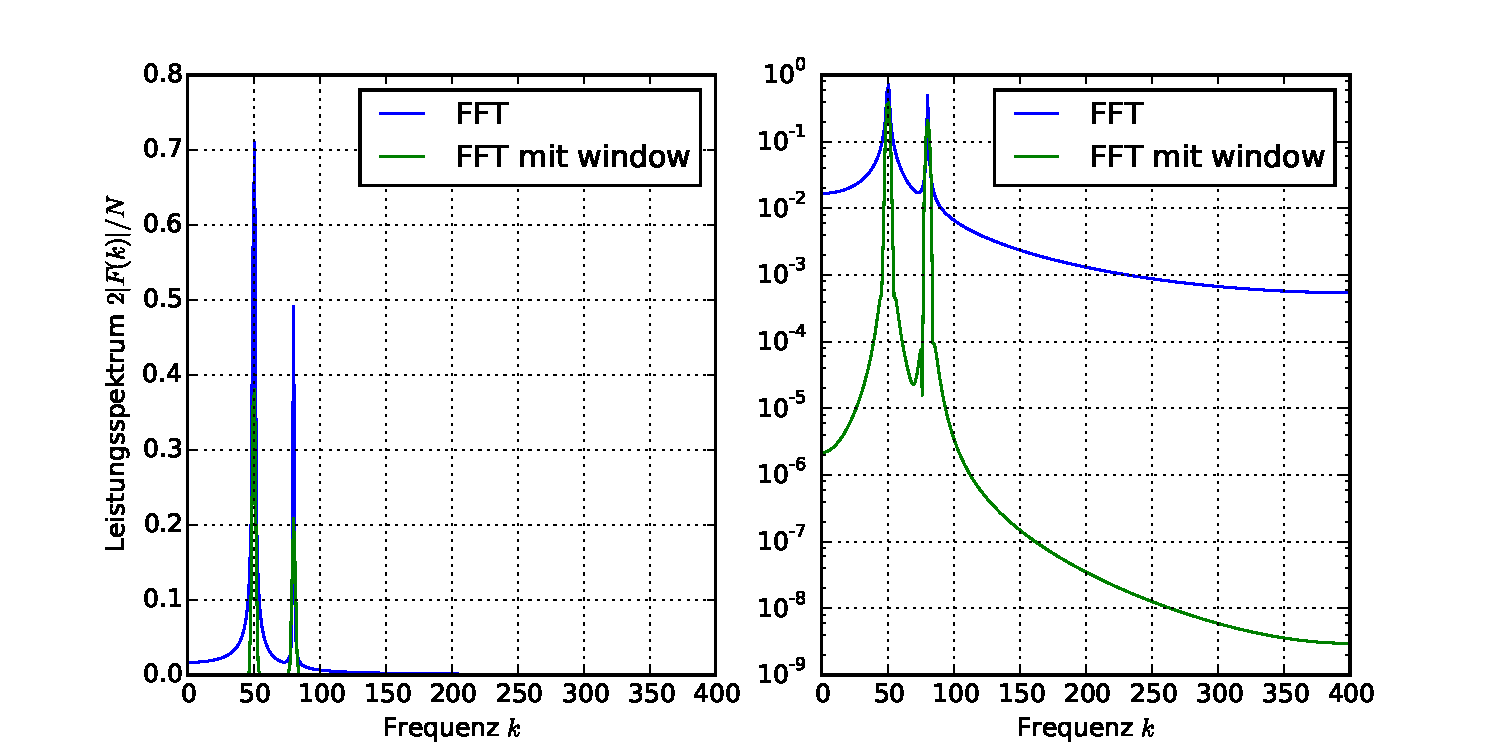
\includegraphics[width=17cm]{pics/stm2}

\section{Anhang: Protokoll des Versuchs}
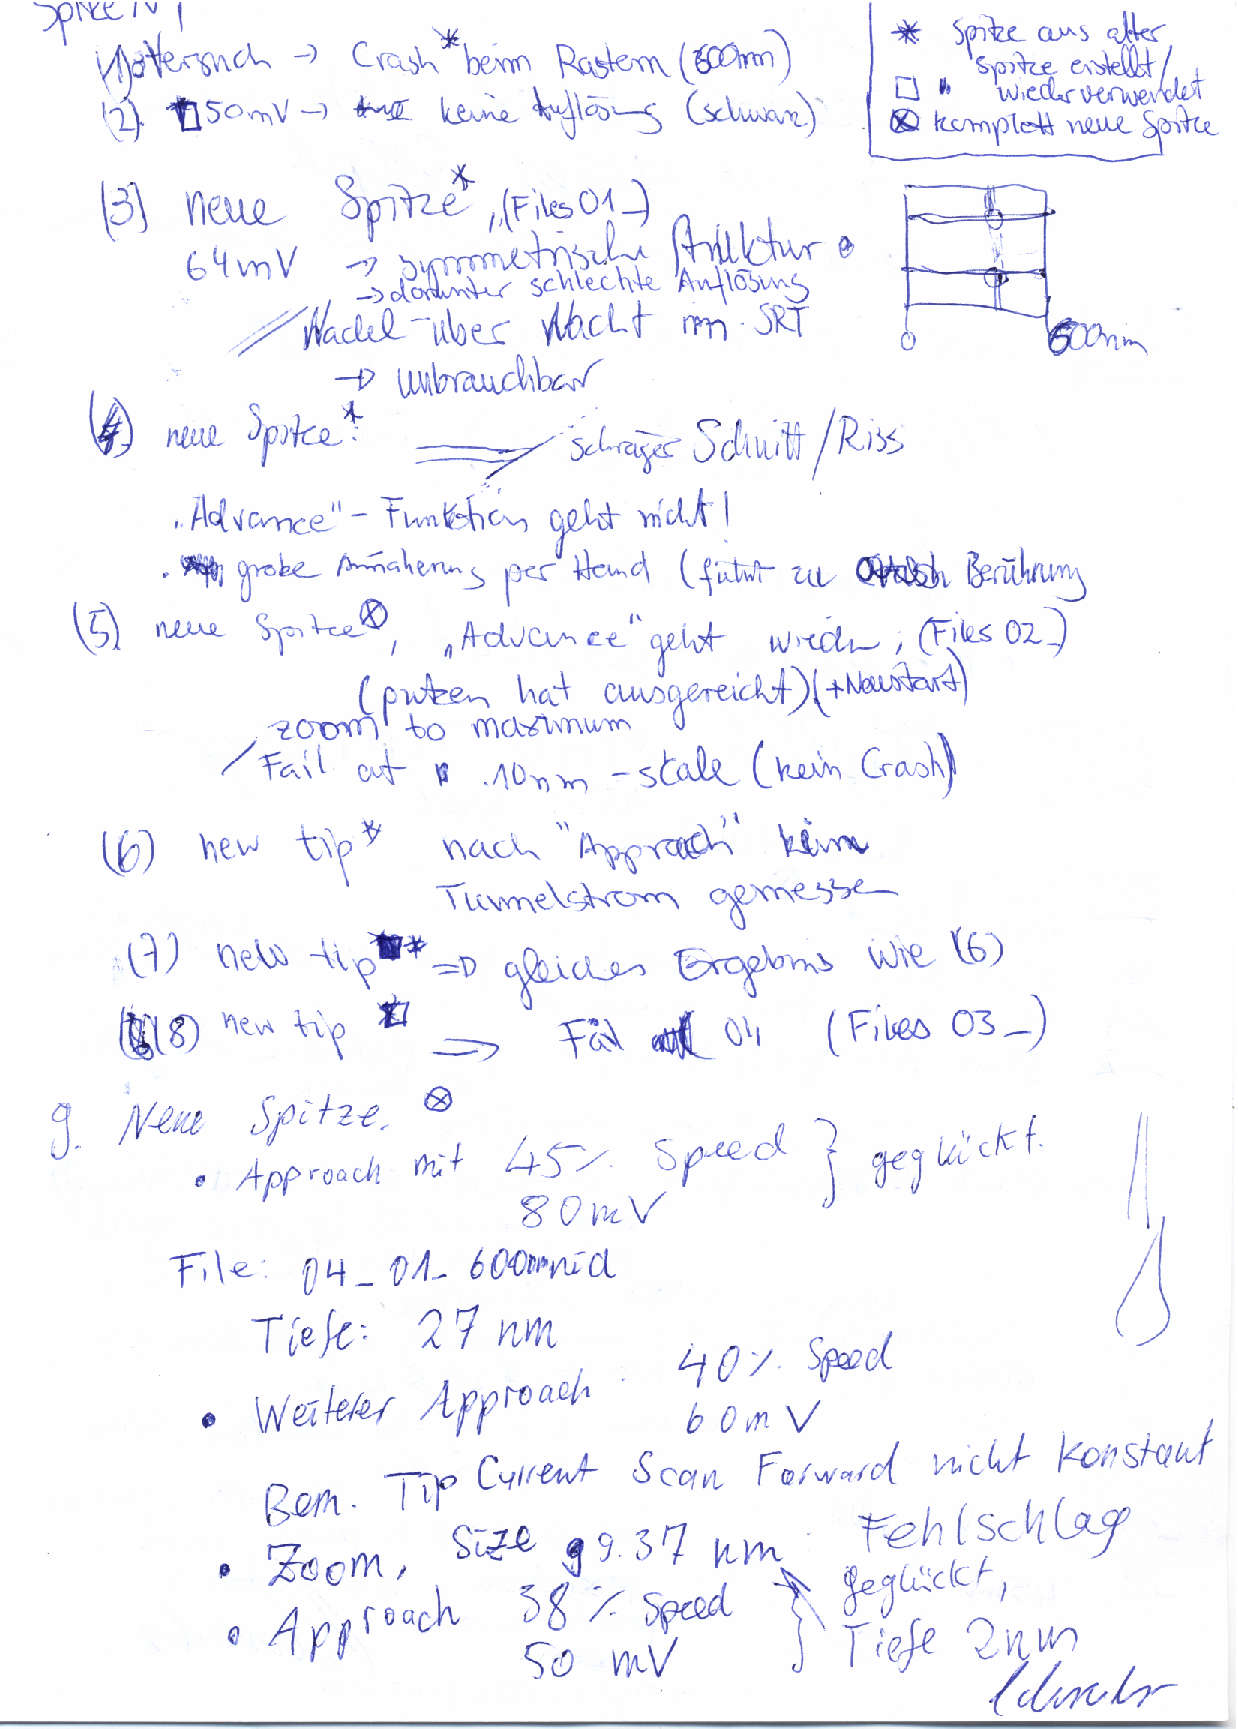
\includegraphics[width=\pagewidth]{protokoll/rtm_protokoll_01}
